\subsection{Frequency dependence of Vertex}


In the next section, we present our result obtained by full frequency dependent fRG. All the results are presented in units of $t=1$.  \textbf{should we write this? repetita iuvat?} 

\paragraph*{Numerical implementation}
We have implemented numerically the flow equations reported in the appendix. 

Due to the different nature of the momentum arguments of self-energy and vertex we have defined two different patching of the irreducible Brillouin zone. 
%The $\phi$-functions depend on a momentum transfer.  
%For the filling and nearest neighbors hopping that we want to describe, the momentum vectors of the most relevant process are $\mathbf{Q}=(0,0)$, important for superconductivity (in the pairing channel) and ferromagnetism (in the magnetic channel); $\mathbf{Q}=(\pi,\pi)$ and its vicinity, relevant for antiferromagnetism and incommensurate antiferromagnetism; the momentum transfer $2k_F$, as defined in Ref.~\onlinecite{Holder2014}, associated to the onset of charge- and spin-density wave instabilities. 
Similarly to what is done in Ref.~\onlinecite{Husemann2009}, the vertex patching describes more accurately the corners around $(0,0)$ and $(\pi,\pi)$, where the instability vectors are expected for our system.

The situation is completely different for the self-energy, for which the most relevant physics happens in the vicinity of the Fermi surface.
% at least in the weak coupling regime. 
Therefore we concentrate the patches along the Fermi surface and in its immediate vicinity (see Fig. \ref{fig:selffermi0600} and Fig. \ref{fig:selffermi0975}), with some further care close to the "antinodal" points near $(\pi,0)$, relevant for antiferromagnetism.
% and pseudogap physics.

%It is not necessary  that the patching-schemes for vertex and self-energy are connected, but the number of patches used should be roughly of the same order.
In the calculations presented in the following we have used $29$ patches for the vertex and $44$ for the self-energy.

For the practical implementation of the frequency dependence we found convenient to rewrite $\mathcal{S}$, $\mathcal{D}$, $\mathcal{C}$ and $\mathcal{M}$ as function of three bosonic frequencies. 
For each frequency argument we restricted ourselves to at least $40$ positive and $40$ negative Matsubara frequencies. 
We stress that the number of Matsubara frequencies that can be taken into account in the calculation sets the lowest reachable temperature.

\subsection{Instabilities analysis}
By means of fRG one can perform an instability analysis of the system: 
for some value of the cutoff $\Lambda$ one of the channels shows a divergence. 
The cutoff scale $\Lambda_{\mathrm{c}} $ for which this happens is called \textit{critical scale}, and from the diverging channel one can evince the leading instability of the system. 
\begin{figure}
\includegraphics[width=0.5\textwidth]{images/phasediag.png}
\caption{Critical scale $1-\Lambda_{\mathrm{c}}$ as a function of the doping $x=1-n$, for $T = 0.08t$, $t'=-0.32t$ and $U=4t$. 
Square symbols and circles refer to incommensurate antiferromagnetism (iAF), respectively without and with self-energy feedback.
The black stars refer to a divergence in the charge channel (forward scattering in Ref. \onlinecite{Husemann2012}). 
The color of squares and circles encodes the distance of the incommensurability vector from $(\pi,\pi)$: darker color corresponds to higher incommensurability. 
The vertical light blue line marks the van Hove filling.}  
\label{fig:criscale} 
\end{figure}
In Fig. \ref{fig:criscale} we show the critical scale $1-\Lambda_{\mathrm{c}}$ as a function of the doping $x=1-n$ with and without self-energy feedback,  for $T=0.08t$, $t'=-0.32t$ and  $U=4t$.
We show our result as function of $1-\Lambda$, which vanishes at the end of the flow. 
For the physical interpretation, we can refer, instead, to the rescaled interaction\cite{Honerkamp2004} $\tilde U ^\Lambda$ as discussed in Sec.\ref{sec:cutoff}.  


The critical value has been defined as the scale for which the value of  the larger channels exceeds $200t$. 
We have checked that for these stopping values the flow of the largest channel begins to increase stronger than exponentially. These results are also consistent with an instability analysis based on the susceptibilities.        

A divergence in the vertex signals a symmetry breaking at finite temperature. This is a consequence of the truncation scheme, that does not respect the Mermin-Wagner theorem\cite{Mermin1966}.
 %since in our truncation-scheme we do not include the bosonic-fluctuations of the order parameter\cite{Baier2004}, essetial to obtain a vanishing critical temperature. 
The presence of a finite critical scale in the pure fermionic fRG signals the appearance of strong bosonic fluctuations that cannot be treated within the approximation-scheme we are using.\cite{Salmhofer2001} 
Even though the flow cannot be continued beyond the critical scale, from the analysis of vertex and self-energy we can identify the more relevant interactions of the system.

%In the specific case of the interaction cutoff we can interprete the rescaled interaction $\tilde U^{\Lambda_\mathrm{c}}$ as the critical interaction at a given temperature.
For the parameter sets shown in Fig.~\ref{fig:criscale} and without self-energy feedback (square and star symbols), there are two possible instabilities. 
For doping smaller than $0.35$ the leading fluctations of the system are either commensurate or incommensurate antiferromagnetic.
The incommensurability $\delta$ is defined through $\mathbf{Q}=(\pi,\pi-\delta)$, where the magnetic channel $\mathcal{M}^\Lambda$ has its maximum for momentum $\bs{Q}$. 
The value of $\delta$ is encoded in the color of the symbols, where darker colors corresponds to larger $\delta$, reaching the value of $\delta=1.13$ for doping $x$ between $0.25$ and $0.35$. 
The region of commensurate antiferromagnetism for  $0.125\le x \le 0.150$ has to be attributed to the presence of a large plateu around $(\pi,\pi)$ in the bare bubble. Correspondingly the magnetic susceptibility is enhanced in all the region around $(\pi,\pi)$, and the commensurate peak coexists with incommensurate ones of similar magnitude.   
\begin{figure}
\includegraphics[width=0.50\textwidth]{images/chargeproblem_MC_vs_Lambda_fix_occ.png}
\caption{Flow of the maximal value of the charge ($\mathcal{C}$) and magnetic ($\mathcal{M}$) channels as functions of $\Lambda$, for  $x=0.4$, $t'=-0.32$, $U=4t$ and $T=0.08t$.  Top: without self-energy feedback; bottom: with self-energy feedback. }
\label{fig:chargeproblem}
\end{figure}

The most striking feature is the presence of a divergence in the charge channel $\mathcal{C}^\Lambda$ for larger values of doping, marked in Fig. \ref{fig:criscale} by black stars. 
This feature was already observed by Husemmann \textit{et al.} in Ref. \onlinecite{Husemann2009}, where it was named "forward scattering instability". 
Unlike the magnetic channel, the charge channel $\mathcal{C}^\Lambda$ diverges for a finite frequency transfer $\Omega=2\pi/\beta$, which makes the interpretation of the divergence in terms of a physical instability not obvious. 
The frequency structure of the divergent charge channel $\mathcal{C}^\Lambda$ and its origin, will be discussed further in paragraph \ref{sec:per_ladder}.

\begin{figure}
\includegraphics[width=0.50\textwidth]{images/chargeproblem_M_vs_Lambda_diff_occ.png}
\caption{Flow of the maximal value of the  magnetic ($\mathcal{M}$) channel as functions of $\Lambda$, for  $x=0.025$ (top) and $x=0.375$ (bottom). The other parameters are $t'=-0.32$, $U=4t$ and $T=0.08t$. Red symbols: with self-energy feedback; blue symbols: without self-energy feedback. }
\label{fig:selfeffect}
\end{figure}

Including the self-energy feedback results in three effects, as can be seen from the circular symbols in Fig. \ref{fig:criscale} . 
First, the self-energy feedback decreases $1-\Lambda_c$.
Second, the incommensurability vector is also affected, the region of commensurate antiferromagnetism disappears, and one can observe a more regular trend of increasing $\delta$ as the doping is increased.
Third, the divergence in the charge channel is completely suppressed, and the leading instability in the doping region $0.375\le x \le 0.4$ remains of the incommensurate antiferromagnetic type. 
This can be also be seen from Fig.~\ref{fig:chargeproblem}, where we compare the flow of the maximum (of the absolute value) of magnetic and charge channel with and without the self-energy feedback for doping $x=0.4$.
Without self-energy feedback, the charge channel rapidly starts to increase, taking large and negative values.
Due to the charge channel feedback the magnetic channel is reduced.    
The effect of the self-energy to the charge channel is evident, as can be seen from the bottom inset: the charge channel does not diverge during the flow, and it is strongly damped.  
At the same time the magnetic channel is enhanced.

This is confirmed by Fig.~\ref{fig:selfeffect}, where we show the maximum of $\mathcal{M}$ with and without self-energy feedback for $x=0.025$ (top inset) and $x=0.375$ (bottom inset).  
One can see that the enhancement of $\mathcal{M}$ due to self-energy is specific of the large doping region, while, in the small doping region the self energy decreases $\mathcal{M}$.  
Hence the self-energy affects the magnetic channel either directly, reducing the particle-hole bubble (for small doping), or indirectly through the feedback of other channels, i.e., reducing the charge channel at large doping. 


\begin{figure}
%\hspace*{-1.5cm}
\includegraphics[width=0.5\textwidth]{images/occupations_0975.png}
\caption{\textbf{placeholder}} 
\label{fig:occ600}
\end{figure}

\begin{figure}
\includegraphics[width=0.5\textwidth]{images/occupations_0600.png}
\caption{\textbf{placeholder} here we will write a lot of useful comments about the figure and I will add a lot of } 
\label{fig:occ975}
\end{figure}


To understand better these effects we looked for possible changes in the Fermi surface structure, analyzing the momentum resolved occupation, computed as: 
\begin{equation}
 n(\mathbf{k})  = \frac{2}{\beta} \sum_{\nu}\frac{e^{i\nu 0^+}}{i\nu-\varepsilon_\bs{k}-\mu^\Lambda-\Lambda\Sigma^\Lambda(\bs{k},i\nu)},\label{eq:occ} 
\end{equation}
where the factor $2$ accounts for the spin degree of freedom. 
In Fig.~\ref{fig:occ975} we show the non interacting (top left) and interacting (top right) occupation in the first quadrant of the Brillouin zone for doping $x=0.025$.
The former is computed by setting $\Sigma^\Lambda=0$ (and non interacting chemical potential) in Eq.(\ref{eq:occ}), while the latter is computed at the critical scale $\Lambda_c$. 
The non interacting Fermi surface broadening is only due to finite temperature.

Comparing the two panels, one does not observe any relevant shift of the Fermi surface location, but the Fermi surface broadening is appreciably larger in the interacting case, due to self-energy.
Similar considerations apply for doping $x=0.4$, as one can see from Fig.~\ref{fig:occ600}, where the broadening is even more evident.  

\begin{figure}
\hspace*{-1.0cm}
\includegraphics[width=0.52\textwidth]{images/Phi_color_all.png}
\caption{Frequency structure of the charge channel $\mathcal{C}^\Lambda_{\Omega,\bs{Q}}(\nu_1,\nu_2)$ (on the left) and of the magnetic channel $\mathcal{M}^\Lambda_{\Omega,\bs{Q}}(\nu_1,\nu_2)$ (on the right), for $x=0.4$, $t'=-0.32$, $U=4t$ and $T=0.08t$ and without self-energy, corresponding to the rightmost point in Fig. \ref{fig:criscale}. 
Both channels are plotted for the frequency and momentum transfer for which they have their maximum. Note that the frequency transfer for $\mathcal{C}^\Lambda_{\Omega,\bs{Q}}$ is the first bosonic Matsubara frquency $2\pi/\beta$. 
The value of $\delta$ is $1.13$.  
 }  
\label{fig:freqplot} 
\end{figure}

\subsection{Vertex frequency dependence}

We focus now on the frequency dependence of the channels. 
In particular we will look at the channels that show a divergence, i.e., the charge and the magnetic observed in Fig.~\ref{fig:criscale}, while we refer to the Appendix for the superconducting ones.

As mentioned in the previous section the divergence of the charge and magnetic channel are different. The charge channel diverges for a finite frequency transfer and only when we neglect the self-energy feedback. 
We will further argue here that the two divergences are also of physical different origin.  

While the dependence on the transfer momentum and frequency $(\bs{Q},\Omega$) has already been studied, here we focus on the dependence on the fermionic frequencies $\nu_1$ and $\nu_2$. 
Therefore we present different color plots for fixed  $(\mathbf{Q},\Omega)$, showing the dependence on the fermionic frequencies. 
 
In the top left panel of Fig.~\ref{fig:freqplot} we show the magnetic channel $\mathcal{M}^{\Lambda_c}_{\mathbf{Q}\Omega}(\nu_1,\nu_2)$ in the small doping region, where antiferromagnetism is leading. 
The case shown has been calculated with self-energy feedback, but we notice that the frequency structures we discuss do not depend strongly on the self-energy feedback. For clarity we restrict the plots to the first $20$ positive and negative Matsubara frequencies, and we notice that larger frequencies can be deduced by the asymptotic.\ref{Wentzell2017}
It is easy to see that the fRG equations are equivalent to RPA when only one channel is taken into account. 
The magnetic channel calculated with RPA would depend only on the frequency and momentum transfer, that would result, for the plot shown, in a completely constant color.
Hence any variation in the frequency structure has to be ascribed to the presence of the other channels in fRG.
As already observed in the literature \textit{who should we cite}, the channel competition suppresses the magnetic channel. 
This is clear in two ways:the largest value of $\mathcal{M}$ is decreased compared to RPA, and the frequency structure at the center is negative compared to the asymptotic value. 

In the bottom left panel of Fig.~\ref{fig:freqplot} we show the charge channel $\mathcal{C}^{\Lambda_c}_{\bs{Q},\Omega}(\nu_1,\nu_2)$ for the same parameter set as before, but for finite frequency transfer $\Omega=2\pi/\beta$, important for the forward scattering instability. 
The frequency structure is completely different from the case described above. 
The channel assumes negative values, and the maximum is for frequencies $\nu_1 = \pi/\beta$ and $\nu_2=-\pi/\beta$. 
This structure cannot be explained in terms of standard ladder diagrams, and might be also related to the behavior of the retarded interaction described by \cite{Stepanov2016}. 

In the two right panels of Fig.~\ref{freplot} we show the same quantities but for $x=0.4$, without self-energy feedback, for which the charge channel has the largest absolute value.  
The frequency structure are similar to the one described above. 
However the maximum (in absolute value) observed in the charge channel is very localized, unlike for the magnetic channel in the iAF case. 	

\paragraph*{Perpendicular ladder} 

 

 



\begin{figure*}
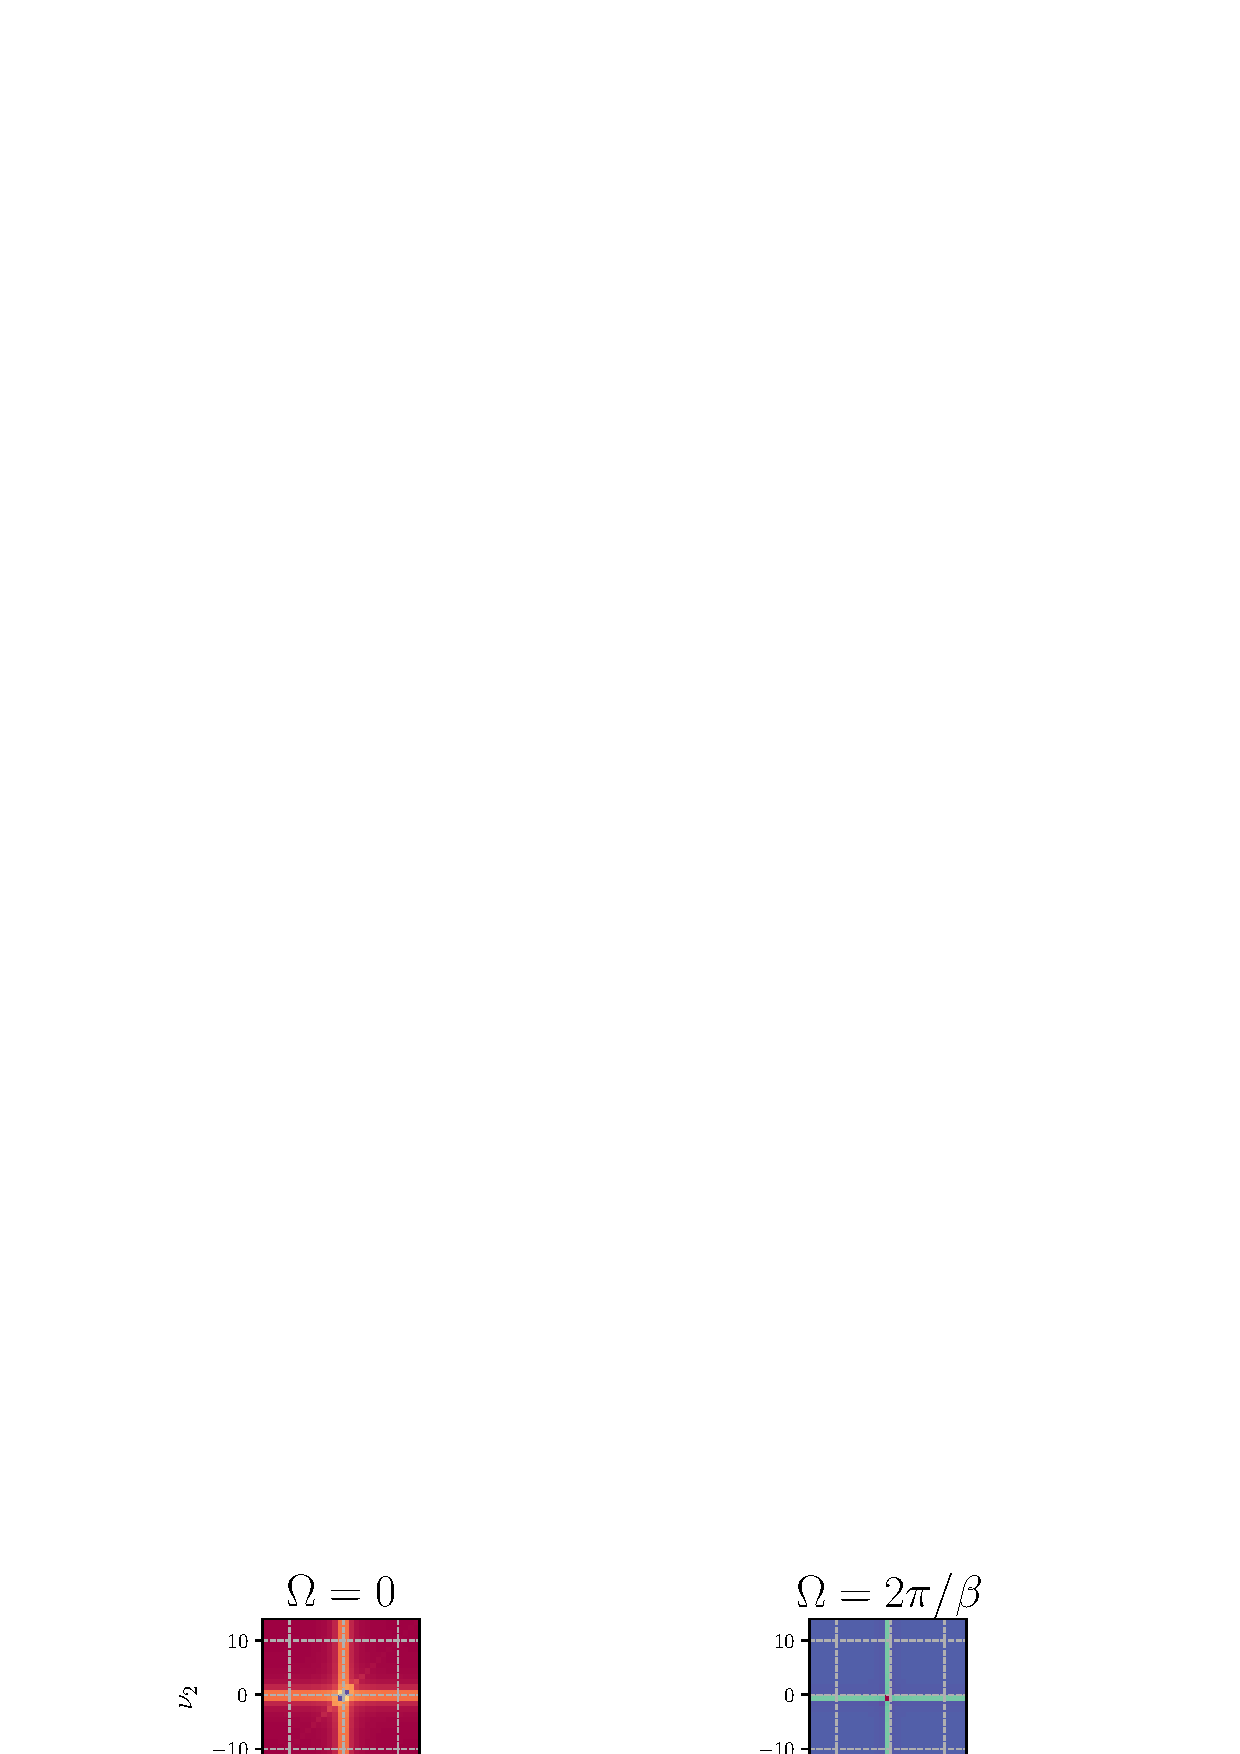
\includegraphics[width=\textwidth]{images/PL_all.png}
\vspace*{-2.0cm}
\caption{\textbf{placeholder}here we will write a lot of useful comments about the figure and I will add a lot of bestemmie} 
\label{fig:perpladder}
\end{figure*}


\begin{itemize}

\item Introduce perpendicular ladder (PL) for charge.

\item Colorplot of charge in PL.

\item Discuss the role of the Bubble at $\boldsymbol{Q}=(0,0)$ and plot it as a function of $\nu$.

\end{itemize}

All these considerations suggest that the divergence of the charge channel is rather an artefact of fRG without self-energy, arising from a lack of consistence between the vertex and the Green's function in the flow equations. 
In the next section we further substanciate this conclusion, by explaining the mathematical origin of the feature. 
The self-energy has qualitative and quantitive effects on the flow equations: quantitively 
\subsection{Self energy analysis}


\begin{figure}
\includegraphics[width=0.50\textwidth]{images/Self_Im_occ0600.png}
\caption{Frequency dependent self-energy for parameter set... .
The location of the $\mathbf{k}$-point in the Brillouin zone is color coded in the inset. }
\label{fig:selffermi0600}
\end{figure}


\begin{figure}
\includegraphics[width=0.50\textwidth]{images/Self_Im_occ0975.png}
\caption{Frequency dependent self-energy for parameter set... .
The location of the $\mathbf{k}$-point in the Brillouin zone is color coded in the inset. }
\label{fig:selffermi0975}
\end{figure}



\begin{figure}
\includegraphics[width=0.5\textwidth]{images/z_and_gamma975.png}
\caption{\textbf{placeholder} }
\label{fig:zetaandgamma}
\end{figure}

\begin{itemize}

\item With self energy feedback, we didn't find any charge instability problem for any parameters range studied.

\item Plot of the Fermi surface based patch scheme.

\item Plot of $\Sigma(i\omega)$ at $\boldsymbol{k}=(\pi,0)$, $\boldsymbol{k}=\boldsymbol{k}_{HS}$ and $\boldsymbol{k}=(\pi/2,\pi/2)$ in frequency space.

\item Plot of $Z_{\boldsymbol{k}}$

\item Plot of occupation with and without $\Sigma$

\end{itemize}
